
\section{Giải pháp ý niệm cho task Route planning và Sequence diagram mô tả nó}
    \subsection{Giải pháp ý niệm cho task Route Planning}
        \textbf{Xét các Actor: }

        \begin{itemize}
            \item[-] Back Officer.
            \item[-] Cơ sở dữ liệu bản đồ (Map Database): một API cung cấp mọi thông tin về đường đi trong một vùng không gian nhất định khi được yêu cầu.
        \end{itemize}

        \textbf{Giả định:}

        \begin{itemize}
            \item[-] Back Officer đã đăng nhập thành công vào hệ thống.
            \item[-] Back Officer đã thao tác với hệ thống, đã nạp một danh sách các MCPs mà mình có nhu cầu tìm đường.
            \item[-] Map Database luôn hoạt động và hoạt động đúng kỳ vọng.
        \end{itemize}

        \textbf{Ta có, các entity liên quan:}

        \begin{itemize}
            \item[-] UIController: Hệ thống đảm nhiệm chức năng làm cầu nối, cho phép người dùng quản lý, sử dụng hệ thống.
            \item[-] RoutePlannerObject: Hệ thống đảm nhiệm chính chức năng tìm đường tự động và đánh giá đường đi.
        \end{itemize}

        \textbf{Các thao tác có thể thực hiện}

        \begin{itemize}
            \item[-] Back officer ra lệnh cho hệ thống tự tạo đường đi (route) phù hợp.
            \item[-] Back officer tự chỉnh sửa, thêm bớt các tuyến đường trong route mới hoặc route đã định sẵn từ thao tác trên.
        \end{itemize}

        \textbf{Mô tả chi tiết các thao tác}
        \begin{enumerate}
            \item Back officer ra lệnh cho hệ thống tự tạo đường đi (route) phù hợp.
            \begin{itemize}
                \item[-] Người dùng thực hiện lệnh tạo route tự động bằng cách ra lệnh GenerateRoute () lên hệ thống.
                \item[-] UIController nhận lệnh, thực hiện lệnh PlanRoute (MCPs, vehicles) lên hệ thống RoutePlannerObject với MCPs, vehicles là các MCP và phương tiện được dùng.
                \item[-] RoutePlannerObject thực hiện GetAvailablePaths (locations, vehicles) đối với Map Database để lấy đường đi hợp lệ giữa các vị trí của MCP mà phương tiện có thể di chuyển qua.
                \begin{itemize}
                    \item[+] Nếu tồn tại những đường đi hợp lệ, RoutePlannerObject tính toán route tốt nhất và trả về cho UIController. UIController trình thông tin về người dùng. Quá trình tự động tạo route kết thúc thành công.
                    \item[+] Nếu không tồn tại path nào, RoutePlannerObject trả về lỗi không tồn tại đường đi cho UIController. Quá trình tự động tạo route kết thúc không thành công.
                \end{itemize}
            \end{itemize}

            \item Back officer tự chỉnh sửa, thêm bớt các tuyến đường trong route mới hoặc route đã định sẵn từ thao tác trên.
            \begin{itemize}
                \item[-] UIController tự chờ mỗi khi người dùng chỉnh sửa, thêm/ bớt route trên giao diện, chạy lệnh ModifyRoute (route) với route là tổng hợp các route mới (mà người dùng đã thay đổi/ chỉnh sửa).
                \item[-] UIController tìm các path có trong route mới, qua lệnh ValidateRoute (paths, MCPs, vehicles) gửi paths vừa chỉnh sửa cho hệ thống RoutePlannerObject để đánh giá tính hợp lệ và hiệu quả.
                \item[-] RoutePlannerObject lấy những đường đi hợp lệ cho phương tiện giữa các MCP từ hệ cơ sở dữ liệu bản đồ bằng lệnh GetPathsBetween (locations, vehicles).
                \item[-] RoutePlannerObject đánh giá nếu đường đi trong route có hợp lệ so với các paths trên bản đồ.
                \begin{itemize}
                    \item[+] Nếu route là hợp lệ, trả về UIController độ hiệu quả của route. UIController trình thông tin đến người dùng và lưu route vào hệ thống. Quá trình chỉnh sửa/ thay đổi route thành công.
                    \item[+] Nếu route là không hợp lệ, trả về UIController sự hợp lệ của route. UIController trình thông tin đến người dùng, không lưu route mới vào hệ thống. Quá trình chỉnh sửa/ thay đổi route không thành công.
                \end{itemize}
            \end{itemize}
        \end{enumerate}
    \subsection{Sequence diagram mô tả giải pháp cho task Route Planning}
        \begin{figure}[H]
            \centering
            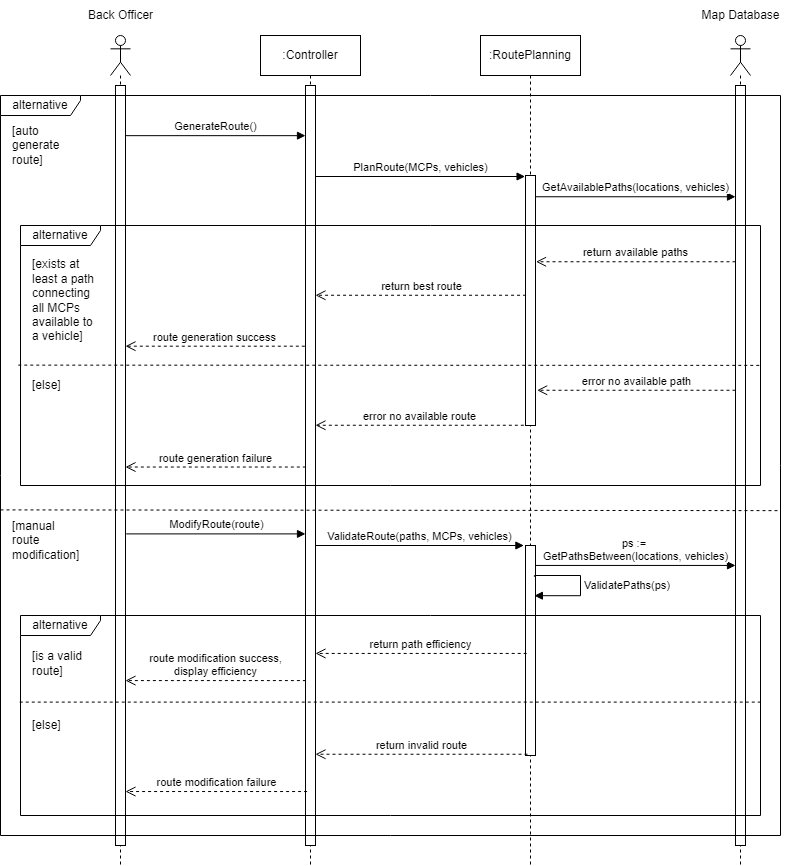
\includegraphics[width=1\linewidth]{imgs/sequence diagram/Sequence Diagram 2.2.png}
            \caption{Sequence diagram cho Task Route Planning}
        \end{figure}

        \newpage
